\documentclass[aspectratio=169]{beamer}

\usetheme{Boadilla}
\usefonttheme{professionalfonts}
\setbeamertemplate{navigation symbols}{}
\setbeamertemplate{itemize items}[circle]
\setbeamertemplate{enumerate items}[default]
\setbeamertemplate{headline}{}

\usepackage[utf8]{inputenc}
\usepackage[T1]{fontenc}
\usepackage{lmodern}
\usepackage{amsmath}
\usepackage{booktabs}
\usepackage{tabularx}
\usepackage{array}
\usepackage{hyperref}
\usepackage[strings]{underscore}
\usepackage{listings}
\usepackage{tikz}
\usetikzlibrary{arrows.meta,positioning,fit,calc,shapes.geometric}
\usepackage{xcolor}

\definecolor{courseblue}{HTML}{12355B}
\definecolor{coursegold}{HTML}{C98A2E}
\definecolor{courseice}{HTML}{EEF3F8}
\definecolor{coursegreen}{HTML}{2F6B4F}
\definecolor{coursegray}{HTML}{4B5563}
\definecolor{codebg}{HTML}{F7F9FC}
\definecolor{codecomment}{HTML}{5E6C84}
\definecolor{codestring}{HTML}{0B6E4F}

\setbeamercolor{palette primary}{bg=courseblue,fg=white}
\setbeamercolor{palette secondary}{bg=coursegold,fg=white}
\setbeamercolor{palette tertiary}{bg=courseblue,fg=white}
\setbeamercolor{palette quaternary}{bg=coursegold,fg=white}
\setbeamercolor{structure}{fg=courseblue}
\setbeamercolor{frametitle}{bg=courseice,fg=courseblue}
\setbeamercolor{title}{fg=courseblue}
\setbeamercolor{block title}{bg=courseblue,fg=white}
\setbeamercolor{block body}{bg=courseice,fg=black}
\setbeamercolor{normal text}{fg=black,bg=white}
\setbeamercolor{alerted text}{fg=coursegold}

\setbeamerfont{footline}{size=\scriptsize}

\setbeamertemplate{footline}{
  \leavevmode
  \hbox{
    \begin{beamercolorbox}[wd=.33\paperwidth,ht=2.8ex,dp=1.2ex,leftskip=0.8em]{palette primary}%
      University of Trieste
    \end{beamercolorbox}%
    \begin{beamercolorbox}[wd=.49\paperwidth,ht=2.8ex,dp=1.2ex,center]{palette tertiary}%
      \coursename{} \textbar{} \coursecode
    \end{beamercolorbox}%
    \begin{beamercolorbox}[wd=.18\paperwidth,ht=2.8ex,dp=1.2ex,rightskip=0.8em plus1fil]{palette secondary}%
      \insertframenumber{} / \inserttotalframenumber
    \end{beamercolorbox}%
  }
}

\hypersetup{
  colorlinks=true,
  linkcolor=courseblue,
  urlcolor=coursegreen
}

\lstdefinestyle{coursepython}{
  language=Python,
  basicstyle=\ttfamily\footnotesize,
  keywordstyle=\color{courseblue}\bfseries,
  commentstyle=\color{codecomment}\itshape,
  stringstyle=\color{codestring},
  showstringspaces=false,
  columns=fullflexible,
  keepspaces=true,
  frame=single,
  framerule=0.6pt,
  rulecolor=\color{courseblue},
  backgroundcolor=\color{codebg},
  xleftmargin=0.4em,
  xrightmargin=0.4em,
  aboveskip=0.4em,
  belowskip=0.2em
}

\newcommand{\coursename}{Data-driven Systems Engineering}
\newcommand{\coursecode}{440MI / 305SM}
\newcommand{\coursefooter}{}

\newcommand{\learninggoals}[1]{
  \begin{block}{Learning goals}
  #1
  \end{block}
}

\newcommand{\repoactivity}[1]{
  \begin{block}{Repo activity}
  #1
  \end{block}
}

\newcommand{\readinglist}[1]{
  \begin{block}{Papers and materials}
  {\footnotesize #1}
  \end{block}
}

\newcommand{\coursecontextframe}[5]{
  \begin{frame}{Course Map and Running Cases}
  \centering
  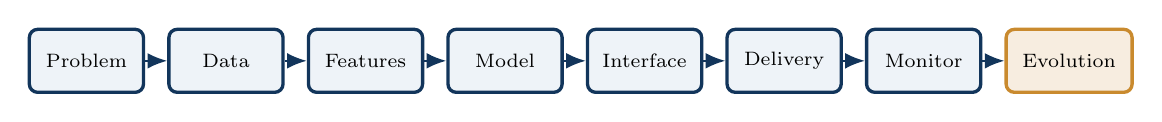
\begin{tikzpicture}[node distance=0.28cm]
  \node[flowbox, minimum width=1.45cm, minimum height=0.8cm] (problem) {\scriptsize Problem};
  \node[flowbox, minimum width=1.45cm, minimum height=0.8cm, right=of problem] (data) {\scriptsize Data};
  \node[flowbox, minimum width=1.45cm, minimum height=0.8cm, right=of data] (features) {\scriptsize Features};
  \node[flowbox, minimum width=1.45cm, minimum height=0.8cm, right=of features] (model) {\scriptsize Model};
  \node[flowbox, minimum width=1.45cm, minimum height=0.8cm, right=of model] (interface) {\scriptsize Interface};
  \node[flowbox, minimum width=1.45cm, minimum height=0.8cm, right=of interface] (delivery) {\scriptsize Delivery};
  \node[flowbox, minimum width=1.45cm, minimum height=0.8cm, right=of delivery] (monitor) {\scriptsize Monitor};
  \node[accentbox, minimum width=1.6cm, minimum height=0.8cm, right=of monitor] (evolution) {\scriptsize Evolution};
  \foreach \a/\b in {problem/data,data/features,features/model,model/interface,interface/delivery,delivery/monitor,monitor/evolution} {
    \draw[arrow] (\a) -- (\b);
  }
  \end{tikzpicture}

  \vspace{0.5em}
  \begin{block}{Today in the course}
  \textbf{Focus:} #1

  \textbf{Bridge:} #2
  \end{block}

  \begin{columns}[T]
  \column{0.48\textwidth}
  \begin{block}{Fraud case}
  {\footnotesize #3}
  \end{block}
  \column{0.48\textwidth}
  \begin{block}{Pasteurization case}
  {\footnotesize #4}
  \end{block}
  \end{columns}

  \vspace{0.3em}
  {\footnotesize \textbf{Course thread:} #5}
  \coursefooter
  \end{frame}
}

\newcommand{\classclosingframe}[4]{
  \begin{frame}{From This Class to the Next}
  \begin{block}{What stays with us}
  #1
  \end{block}

  \begin{columns}[T]
  \column{0.48\textwidth}
  \begin{block}{Project use}
  {\footnotesize #2}
  \end{block}
  \column{0.48\textwidth}
  \begin{block}{Next connection}
  {\footnotesize #3}
  \end{block}
  \end{columns}

  \vspace{0.3em}
  {\footnotesize \textbf{Course thread:} #4}
  \coursefooter
  \end{frame}
}

\tikzset{
  flowbox/.style={
    rounded corners=3pt,
    draw=courseblue,
    fill=courseice,
    very thick,
    minimum width=2.2cm,
    minimum height=0.9cm,
    align=center,
    font=\small
  },
  accentbox/.style={
    rounded corners=3pt,
    draw=coursegold,
    fill=coursegold!15,
    very thick,
    minimum width=2.2cm,
    minimum height=0.9cm,
    align=center,
    font=\small
  },
  arrow/.style={
    -{Latex[length=2.5mm,width=2mm]},
    thick,
    draw=courseblue
  }
}


\title{Class 19: Lab -- Streaming Pasteurization Sensors}
\author{\coursename}
\date{}

\begin{document}

\frame{\titlepage \coursefooter}

\begin{frame}{Agenda}
\begin{itemize}
\item Lab goal: go from synthetic sensor generation to a live stream you can consume.
\item Walk through `synth_sensors.py`: states, sensors, and the derived `dTdt` feature.
\item Walk through `serving.py`: batch, point, and streaming endpoints.
\item Guided exercises: run, inspect, request, and stream.
\item What to observe, and common pitfalls.
\end{itemize}
\coursefooter
\end{frame}

\begin{frame}{Learning goals}
\learninggoals{
\begin{itemize}
\item Run the pasteurization synthetic sensor generator and inspect its output.
\item Explain how a Flask endpoint turns a batch simulation into a live stream.
\item Connect the state machine from Class 13 to actual code that implements it.
\item Practice validating a data-generating service before trusting anything built on top of it.
\end{itemize}
}
\coursefooter
\end{frame}

\coursecontextframe
{Hands-on practice: generating and serving the streaming sensor case end to end.}
{This is a lab session: it takes the data-type and online-learning ideas from Classes 13 and 18 and turns them into a running service you operate yourself.}
{The fraud case has no streaming lab counterpart, but the habits practiced here, validating a generator, testing an endpoint, still apply directly to any API-based service.}
{The pasteurization case is the entire subject of this lab: `synth_sensors.py` generates it, `serving.py` streams it.}
{Everything from data types to online learning becomes concrete only once you can run the pipeline that produces the data.}

\begin{frame}{Lab overview and setup}
\begin{enumerate}
\item From the repository root, install dependencies: `pip install -r requirements.txt`.
\item Two files matter today: `pasteurization/synth_sensors.py` and `pasteurization/serving.py`.
\item `synth_sensors.py` has no Flask dependency; it can be run and inspected standalone.
\item `serving.py` imports functions directly from `synth_sensors.py` and exposes them over HTTP.
\end{enumerate}
\coursefooter
\end{frame}

\begin{frame}[fragile]{The sensors and states, in code}
\begin{lstlisting}[style=coursepython]
# Sensors (7): Temperature, pH, Kappa, Mu, Tau, Q_in, Q_out, P
# Derived: dT/dt

PROD_RANGES = {
    "Idle":      (60, 120),
    "Fill":      (30, 60),
    "HeatUp":    (30, 45),
    "Hold":      (15, 25),
    "Cool":      (30, 60),
    "Discharge": (60, 120),
}
\end{lstlisting}
\begin{itemize}
\item From `pasteurization/synth_sensors.py`: seven physical sensors, six production states, each with a randomized duration range in seconds.
\end{itemize}
\coursefooter
\end{frame}

\begin{frame}{The batch lifecycle as a state machine}
\centering
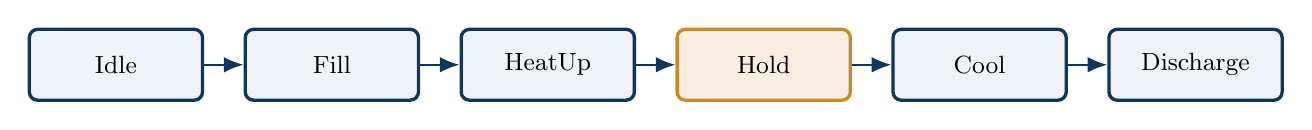
\begin{tikzpicture}[node distance=0.5cm]
\node[flowbox] (idle) {\small Idle};
\node[flowbox, right=of idle] (fill) {\small Fill};
\node[flowbox, right=of fill] (heat) {\small HeatUp};
\node[accentbox, right=of heat] (hold) {\small Hold};
\node[flowbox, right=of hold] (cool) {\small Cool};
\node[flowbox, right=of cool] (disch) {\small Discharge};
\foreach \a/\b in {idle/fill,fill/heat,heat/hold,hold/cool,cool/disch} {
  \draw[arrow] (\a) -- (\b);
}
\end{tikzpicture}
\vspace{0.4em}
\begin{itemize}
\item Every function named `seg\_*` in `synth_sensors.py` implements exactly one of these six boxes.
\end{itemize}
\coursefooter
\end{frame}

\begin{frame}{Exercise 1: generate and inspect a batch}
\begin{enumerate}
\item Run `python synth_sensors.py` from the `pasteurization/` directory.
\item Open the resulting `synthetic_pasteurization_signals.csv` and check the `state` column against the six states above.
\item Plot `T` and `dTdt` for a single `batch_id` and identify the `HeatUp` and `Cool` phases visually.
\item Confirm that `dTdt` changes sign exactly where the temperature trend reverses.
\end{enumerate}
\coursefooter
\end{frame}

\begin{frame}[fragile]{The derived feature, in code}
\begin{lstlisting}[style=coursepython]
def simulate_batch(bid, start_time=0.0):
    ...
    frames = simulate_production_cycle(pdur, ctx)
    df, t = to_df(frames, start_time, bid)
    df["dTdt"] = df["T"].diff().fillna(0.0) / DT
    return df, t
\end{lstlisting}
\begin{itemize}
\item This is the exact construction from Class 15's ``feature construction for streams'' section, now something you run yourself.
\end{itemize}
\coursefooter
\end{frame}

\begin{frame}{Exercise 2: serve a batch over HTTP}
\begin{enumerate}
\item Start the Flask service: `python serving.py` (listens on port 8001).
\item Request a full simulated batch: `GET /batch`.
\item Request a single simulated reading at a chosen time: `GET /point?t=45`.
\item Vary `t` across the six state durations and confirm the returned `state` field changes accordingly.
\end{enumerate}
\coursefooter
\end{frame}

\begin{frame}[fragile]{Serving a single point, in code}
\begin{lstlisting}[style=coursepython]
@app.route("/point")
def point():
    try:
        t = float(request.args.get("t", 0))
    except ValueError:
        return jsonify({"error": "Invalid t parameter"}), 400

    data = simulate_point(t)
    return jsonify(data)
\end{lstlisting}
\begin{itemize}
\item From `pasteurization/serving.py`: input validation (`try`/`except`) is already present here, a good pattern to notice and reuse.
\end{itemize}
\coursefooter
\end{frame}

\begin{frame}{Exercise 3: consume the live stream}
\begin{enumerate}
\item With `serving.py` still running, request `GET /stream` with `curl -N http://localhost:8001/stream`.
\item Observe one JSON event arriving per second, in the Server-Sent Events format.
\item Alternatively, launch `streamlit run streamlit/Main.py` and open the Pasteurization dashboard page, which consumes this same `/stream` endpoint.
\item Compare the raw `curl` output to what the dashboard renders.
\end{enumerate}
\coursefooter
\end{frame}

\begin{frame}[fragile]{The streaming endpoint, in code}
\begin{lstlisting}[style=coursepython]
@app.route("/stream")
def stream():
    df, _ = simulate_batch(BATCH_ID)

    def generate():
        for _, row in df.iterrows():
            yield f"data: {json.dumps(row.to_dict())}\n\n"
            time.sleep(STREAM_DT)

    return Response(generate(), mimetype="text/event-stream")
\end{lstlisting}
\begin{itemize}
\item From `pasteurization/serving.py`: a whole batch is simulated first, then replayed one row per second as a live event stream.
\end{itemize}
\coursefooter
\end{frame}

\begin{frame}{What to observe while streaming}
\begin{itemize}
\item State transitions should follow the fixed order: Idle, Fill, HeatUp, Hold, Cool, Discharge.
\item `dTdt` should be near zero during `Idle` and `Hold`, and clearly non-zero during `HeatUp` and `Cool`.
\item `Q\_in` is only non-zero during `Fill`; `Q\_out` is only non-zero during `Discharge`.
\item Every sensor stays within the fixed y-axis ranges used by the Streamlit dashboard.
\end{itemize}
\coursefooter
\end{frame}

\begin{frame}{Common pitfalls in this lab}
\begin{itemize}
\item Forgetting `threaded=True` when running Flask can make the `/stream` endpoint block other requests.
\item Port conflicts: `serving.py` defaults to 8001; check nothing else is already bound to it.
\item The Streamlit dashboard's sidebar IP and port must match wherever `serving.py` is actually running.
\item `/stream` regenerates a new batch every time it is called; two simultaneous clients will not see identical data.
\end{itemize}
\coursefooter
\end{frame}

\begin{frame}{Repository connections}
\repoactivity{
\begin{itemize}
\item `pasteurization/synth_sensors.py` and `pasteurization/serving.py` are the two files this entire lab is built from.
\item `streamlit/pages/App_Pasteurization.py` is the ready-made client that consumes `/stream` for live plotting.
\end{itemize}
}
\coursefooter
\end{frame}

\begin{frame}{Reflection prompt}
\begin{block}{Question}
What would you change in `synth_sensors.py` to simulate a sensor fault or a slow drift, so that Class 18's ADWIN detector would have something real to catch?
\end{block}
\begin{itemize}
\item There is no single correct answer; the goal is to connect a code change to a detectable statistical effect.
\end{itemize}
\coursefooter
\end{frame}

\begin{frame}{Papers and materials}
\readinglist{
\href{https://flask.palletsprojects.com/en/stable/}{Flask documentation};\
\href{https://flask.palletsprojects.com/en/stable/tutorial/}{Flask tutorial};\
\href{https://docs.streamlit.io/}{Streamlit documentation};\
\href{https://pandas.pydata.org/docs/}{pandas documentation}.
}
\coursefooter
\end{frame}

\classclosingframe
{\begin{itemize}
\item A synthetic generator plus a thin Flask layer is enough to turn a state-machine model into a live, streamable service.
\item Input validation and clear route boundaries are software engineering habits, not extras, even in a small simulation service.
\item Running and probing a service yourself surfaces assumptions that reading the code alone does not.
\end{itemize}}
{Project teams building a streaming or simulation component can reuse this generate-then-serve pattern directly.}
{Class 20 asks how a trained model, not just a data generator, gets served the same way, and bridges into the MLOps block that follows.}
{Whether the payload is a sensor reading or a model prediction, the serving concerns, validation, format, and reliability, are the same.}

\end{document}
